%% ======================================================================
%% 09_validation.tex -- 8. Validation and characterization (+ model validation)
%% ======================================================================
\section{Validation and characterization}
\label{sec:validation}

Validation follows the scenarios defined in the course guide: mobile-base motion on flat ground and on a \SI{10}{\degree} slope, ball balancing with the base stationary and moving, and stability of the intermediate stage (the octocopter). All results come from logs recorded on November 17, 18, 20, and 23, 2026, and published in the repository. Ball error is the Euclidean distance between the ball and the plate center (reference $(0,0)$), computed only while the PID controller was active and the ball was detected.

\subsection{Test methodology and metrics}
\label{sec:metodologia}
The final test protocol (Nov.~23) defined configurations that add \emph{one element at a time}, isolating each error increase to the newly added subsystem:
\begin{itemize}
  \item C0: unpowered measurements (\emph{completed});
  \item C1: ball and plate alone, with the base stationary and the drone off (\emph{completed});
  \item C2: moving base with the drone locked to the base, equivalent to a \emph{servos-only} solution (\emph{pending});
  \item C3: full robot with the drone free on the spherical joint (\emph{completed}).
\end{itemize}
The protocol also includes test~D (comparing C2 and C3 over the same ramp cycle as a direct test of Section~\ref{sec:porquedron}), as well as dedicated tape-measured translation/rotation tests (E1), a sinusoidal plate sweep (E2), recovery from 2 and \SI{5}{\centi\metre} offsets (E3), and weight relief at $f=0.5$. These tests were not executed during the Nov.~23 campaign and remain future work (Section~\ref{sec:limits}). Table~\ref{tab:metricas} summarizes the metrics defined in \texttt{metricas\_pruebas.py} and their measurement status.

\begin{table}[!htbp]
\centering
\small
\caption{Performance metrics, acceptance criteria, and validation status. $e(t)$ is the ball distance to the center, in mm, while the PID is active; $R_u=\SI{96.5}{\milli\metre}$ is the usable plate radius.}
\label{tab:metricas}
\begin{tabularx}{\textwidth}{@{}>{\raggedright\arraybackslash}p{0.23\textwidth}>{\raggedright\arraybackslash}X>{\raggedright\arraybackslash}p{0.22\textwidth}>{\raggedright\arraybackslash}p{0.15\textwidth}@{}}
\toprule
Metric & Definition & Criterion & Status \\
\midrule
Relative error & $e_{\mathrm{RMS}}/R_u\times100$ & E3: $\le\SI{10}{\percent}$ (off), $\le\SI{30}{\percent}$ (idle); E4/E5: $\le\SI{45}{\percent}$ & measured (Table~\ref{tab:ensayos23}) \\
Effectiveness & \% of time with $e\le\SI{30}{\milli\metre}$ (and \SI{50}{\milli\metre} band on Nov.~23) & E3: $\ge\SI{90}{\percent}$; E4/E5: $\ge\SI{60}{\percent}$ & measured (Tables~\ref{tab:ensayos23}--\ref{tab:completos23}) \\
Ball losses and success rate & intervals $>\SI{1}{\second}$ without ball; loss-free / total trials & $\ge\SI{80}{\percent}$ & measured on bench and ramp \\
Recovery (2 and \SI{5}{\centi\metre}) & time to enter band (5 or \SI{20}{\milli\metre}) and stay \SI{2}{\second}; overshoot & $\le$3 and \SI{5}{\second}; success $\ge\SI{80}{\percent}$ & pending (E3) \\
Servo control effort & $\sqrt{\overline{(u_x-n_x)^2+(u_y-n_y)^2}}$ (\si{\micro\second}); activity $\sum|\Delta u|/T$ & compare C1, C2, and C3, and D-A vs.\ D-B & C1/C3 measured; C2 and D pending \\
Servo usage and saturation & mean $\max|u-n|/\SI{220}{\micro\second}$; \% of time $\ge\SI{95}{\percent}$ & saturation $\le\SI{10}{\percent}$ & measured (Nov.~18 and Pi Nov.~23) \\
Drone control effort & spread across the 8 motors (\si{\micro\second}) and mean collective & zero cutoffs in base mode & measured (Secs.~\ref{sec:flights}--\ref{sec:ensayos23}) \\
Base: translation and rotation & $|d-d_{\mathrm{ref}}|/d_{\mathrm{ref}}$ and $|\psi-\SI{360}{\degree}|/\SI{360}{\degree}$ & $\le\SI{5}{\percent}$ & speed and drift measured; 25/50\,cm and \SI{360}{\degree} pending \\
Platform & max frequency with amplitude $\ge\SI{70}{\percent}$ (0.5--\SI{4}{\hertz} sweep) & $\ge\SI{1}{\hertz}$ & pending (E2) \\
\bottomrule
\end{tabularx}
\end{table}

\paragraph{Unpowered measurements (C0, Nov.~23)} These measurements replaced values that the model previously took from CAD or estimates:
\begin{itemize}
  \item total robot mass: \SI{10.4}{\kilo\gram};
  \item wheelbase: \SI{0.22}{\metre};
  \item vertical guide travel: roughly \SI{140}{\milli\metre} (CAD indicated \SI{77}{\milli\metre});
  \item static tip-over angles: \SI{21.5}{\degree} and \SI{30.5}{\degree}, yielding $x_G=\SI{88}{\milli\metre}$ and $h_G=\SI{224}{\milli\metre}$;
  \item spherical joint range: \SI{35}{\degree} toward M8, \SI{40}{\degree} toward M6, \SI{47}{\degree} toward M5, and \SI{53}{\degree} toward M7.
\end{itemize}
The spherical joint range comfortably exceeds the \SI{10}{\degree} base angle change at each ramp transition. Therefore, the Nov.~18 tilt cutoffs upon entering the ramp did not result from the module hitting a mechanical stop. Instead, dynamics explain them: the transition impact excites an inverted pendulum that has low torque authority at idle.

\subsection{Octocopter on the bench (rotors at idle)}
On Nov.~18, the drone operated at a fixed \SI{1300}{\micro\second} collective on the free spherical joint while pushed by hand. The onboard buffer logged data at 190--\SI{200}{\hertz} (Fig.~\ref{fig:bench}).

\begin{itemize}
  \item Across both trials, RMS roll was \SI{0.38}{\degree} and \SI{0.26}{\degree}, and RMS pitch was \SI{0.26}{\degree} and \SI{0.24}{\degree}.
  \item Maximum tilt was \SI{1.42}{\degree}.
  \item Motor commands stayed between \SI{1255}{\micro\second} and \SI{1338}{\micro\second}, indicating low control effort.
  \item After the largest push (\SI{3.7}{\degree}), the drone re-leveled in about \SI{1}{\second}.
\end{itemize}

\begin{figure}[!htbp]
  \centering
  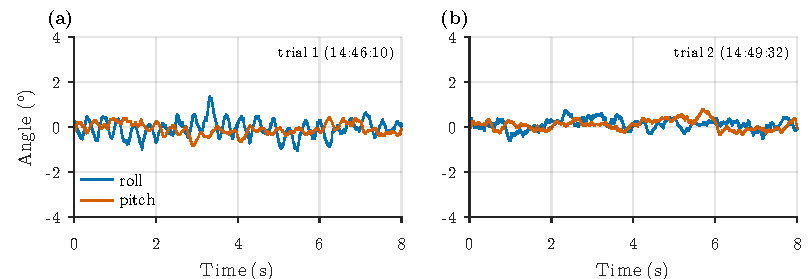
\includegraphics{figures/fig_drone_bench.pdf}
  \caption{Octocopter attitude on the free spherical joint at idle collective (\SI{1300}{\micro\second}), logged onboard at 190--\SI{200}{\hertz}.}
  \label{fig:bench}
\end{figure}

\subsection{Flight campaign on the vertical guide}
\label{sec:flights}
On Nov.~20, nine flights were performed on the vertical guide across successive firmware versions, starting the afternoon session with the LiPo batteries charged to 12.4\,V at rest. Table~\ref{tab:flights} and Fig.~\ref{fig:flights} summarize the campaign.

\begin{itemize}
  \item \textbf{Flights 1--2.} Revealed two issues: accelerometer saturation from rotor vibration (\SIrange{0.03}{2.2}{g}), which triggered false tilt cutoffs, and real yaw rotation of the drone on the spherical joint. These findings led to the \SI{10}{\hertz} accelerometer filter and the yaw loop.
  \item \textbf{Flights 3--6.} Lifted off, then slowly drifted in pitch or roll until the operator or safety interlock stopped them. The drift had a 5--\SI{10}{\second} period and was identical with full gains (v5) and reduced gains (v6). This pointed to the torque-authority limit of Section~\ref{sec:authority}---whose region of attraction was only 3--4$^\circ$---rather than gain tuning.
  \item \textbf{Flight 7} (v8, wider angular-rate limit). First stable hover: \SI{20}{\second} at 1725--\SI{1775}{\micro\second}, with \SI{0.55}{\degree} RMS roll and \SI{1.19}{\degree} RMS pitch. A cutoff occurred during landing when gains reverted to bench values while the drone was still airborne.
  \item \textbf{Flights 8--9} (v9, with hysteresis). Flew and landed without cutoff. In Flight~9, takeoff required \SI{1796}{\micro\second} (\SI{21}{\micro\second} higher than Flight~8) and collective was raised to \SI{1816}{\micro\second}; after \SI{48}{\second} of hovering, pitch diverged to the \SI{12}{\degree} limit. Allocation saturation does not explain this, because \eqref{eq:taumax} still provides \SI{2.4}{\newton\metre}. The candidate causes are the lightly damped slow mode of Section~\ref{sec:attitude}, whose damping depends on $k_T$, and battery voltage sag, which reduces $k_T$ with $V_{\mathrm{bus}}^2$: by the end of Flight~9, each LiPo had delivered \SI{1.0}{\ampere\hour} that afternoon (Section~\ref{sec:bateria}). Later, at 11.1\,V, the module no longer lifted off.
\end{itemize}

\begin{table}[!htbp]
\centering
\caption{Flight campaign on the vertical guide (November 20, 2026). RMS error relative to horizontal, computed while mean motor command exceeded \SI{1650}{\micro\second}.}
\label{tab:flights}
\footnotesize
\setlength{\tabcolsep}{4pt}
\begin{tabularx}{\textwidth}{@{}clrrrrr>{\raggedright\arraybackslash}X@{}}
\toprule
Flight & FW & Max.\ col. & $t$ & Roll & Pitch & Max. & Outcome \\
 & & (\si{\micro\second}) & (\si{\second}) & RMS (\si{\degree}) & RMS (\si{\degree}) & tilt (\si{\degree}) & \\
\midrule
1 & v2 & 1625 & 0 & -- & -- & -- & tilt cutoff (accelerometer vibration) \\
2 & v3 & 1475 & 0 & -- & -- & -- & yaw cutoff ($-20^\circ$) \\
3 & v4 & 1700 & 10.9 & 0.93 & 4.89 & 9.8 & operator stop, pitch drift \\
4 & v5 & 1800 & 19.4 & 2.99 & 0.95 & 9.3 & operator stop, slow oscillation \\
5 & v6 & 1700 & 3.1 & 0.83 & 3.59 & 10.9 & tilt cutoff at takeoff \\
6 & v6 & 1725 & 8.4 & 4.14 & 1.38 & 11.1 & roll cutoff (videos IMG\_1867--1868) \\
7 & v8 & 1775 & 27.2 & 0.55 & 1.19 & 4.3 & \SI{20}{\second} hover; cutoff on landing (video IMG\_1869) \\
8 & v9 & 1775 & 31.0 & 1.15 & 0.95 & 3.8 & hover and landing, no cutoff \\
9 & v9 & 1816 & 62.0 & 1.73 & 1.70 & 10.8 & \SI{48}{\second} hover; pitch cutoff \\
\bottomrule
\end{tabularx}
\end{table}

\begin{figure}[!htbp]
  \centering
  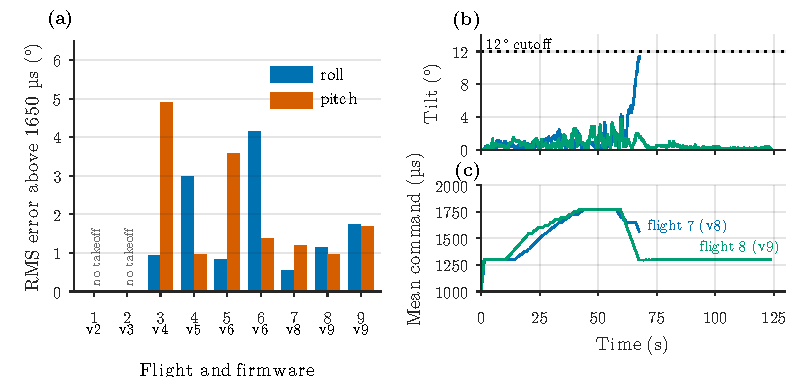
\includegraphics{figures/fig_flight_campaign.pdf}
  \caption{Flight campaign on the vertical guide. (a) RMS roll and pitch error above \SI{1650}{\micro\second} for each flight, with firmware version. (b) Tilt and (c) mean motor command for Flights~7 (v8) and 8 (v9): v8 cuts off when flight gains deactivate during landing, whereas v9 lands normally.}
  \label{fig:flights}
\end{figure}

\paragraph{Videos synchronized with telemetry}
The three Nov.~20 videos (iPhone, 4K at \SI{120}{fps}) were synchronized with the logs using the file creation timestamp (which marks recording start on iPhone) and the PC timestamp on each log line (Fig.~\ref{fig:video}). IMG\_1867 (15:10:11, \SI{11}{\second}) shows Flight~6 as the collective ramps from 1600 to \SI{1675}{\micro\second}. IMG\_1868 (15:10:26, \SI{4}{\second}) captures its end: roll moves from $-6^\circ$ to $-11.1^\circ$ in \SI{1.3}{\second}, the firmware cuts the motors, and the module drops onto the guide, matching the log within \SI{1}{\second}. IMG\_1869 (15:23:32, \SI{13}{\second}) falls inside the Flight~7 hover, with collective between 1763 and \SI{1775}{\micro\second} and tilt between 0.1 and 1.7$^\circ$. In all three videos, an operator follows the camera mast by hand as a safety measure; the footage cannot rule out light contact, which would act as an additional disturbance on the attitude loop; the figures in Table~\ref{tab:flights} are reported directly from the logs.

\begin{figure}[!htbp]
  \centering
  \begin{subfigure}[b]{0.24\textwidth}\centering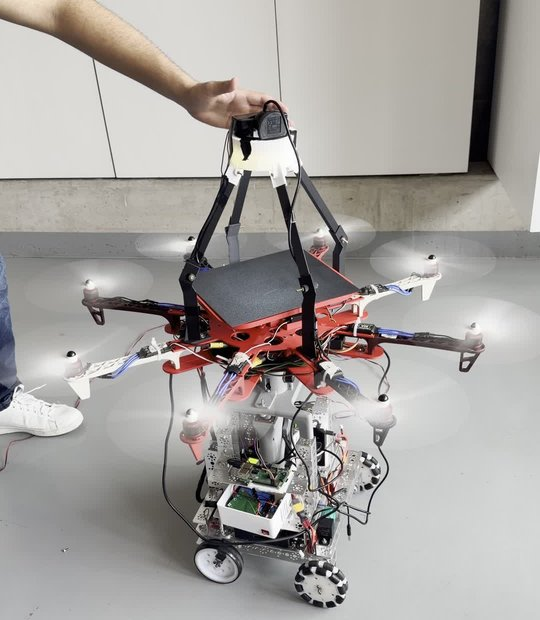
\includegraphics[width=\linewidth]{figures/video_a.jpg}\caption{Flight~6, \SI{1650}{\micro\second}.}\end{subfigure}\hfill
  \begin{subfigure}[b]{0.24\textwidth}\centering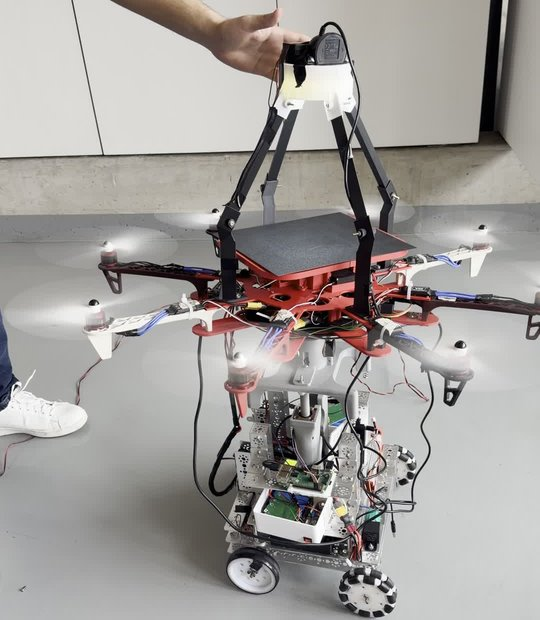
\includegraphics[width=\linewidth]{figures/video_b.jpg}\caption{Flight~6, \SI{1724}{\micro\second}.}\end{subfigure}\hfill
  \begin{subfigure}[b]{0.24\textwidth}\centering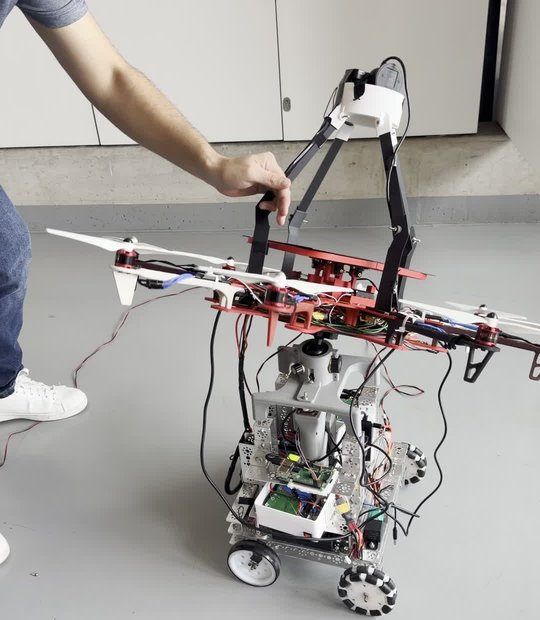
\includegraphics[width=\linewidth]{figures/video_c.jpg}\caption{Flight~6, after cutoff.}\end{subfigure}\hfill
  \begin{subfigure}[b]{0.24\textwidth}\centering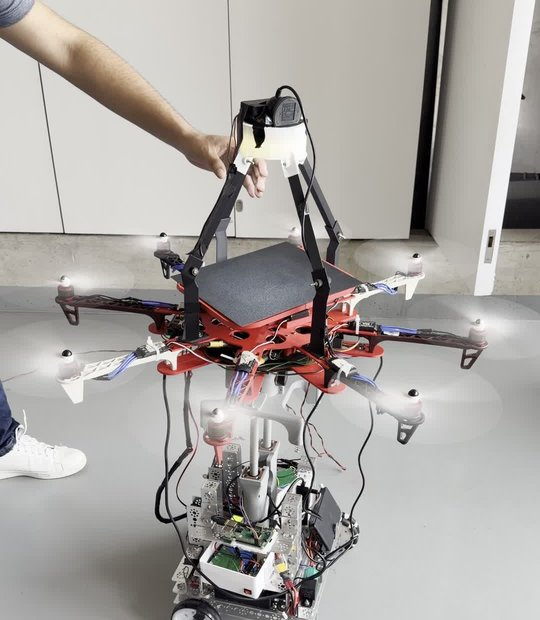
\includegraphics[width=\linewidth]{figures/video_d.jpg}\caption{Flight~7, \SI{1774}{\micro\second}.}\end{subfigure}
  \caption{Frames from the Nov.~20 videos synchronized with telemetry: (a) IMG\_1867 at \SI{6}{\second}, (b) IMG\_1868 at \SI{1}{\second}, (c) IMG\_1868 at \SI{3.2}{\second}, after the $-11.1^\circ$ roll cutoff with motors stopped and the module resting on its side, and (d) IMG\_1869 at \SI{7}{\second}, hovering at 0.4--0.6$^\circ$ tilt. The LiPo batteries were near 12.4\,V.}
  \label{fig:video}
\end{figure}

\paragraph{Comparison with the Isaac Lab model}
Before testing, the assembly was modeled in Isaac Lab \cite{mittal2023} from CAD, including the spherical joint and vertical guide (\SI{3.6}{\kilo\gram}, thrust capped at \SI{6}{\newton} per motor). Both a PPO policy \cite{schulman2017} and a classical PI-D controller were trained and evaluated there. Comparison yields two distinct findings:
\begin{itemize}
  \item \textbf{Thrust.} The model predicted hover at \SI{1899}{\micro\second} (\SI{4.41}{\newton} per motor); the physical assembly lifted off 124--\SI{174}{\micro\second} earlier, meaning the actual thrust gain is 33--52\% higher (Section~\ref{sec:ident}). The thrust model was conservative, and that error---not controller tuning---placed the physical attitude loop inside the stable region of Fig.~\ref{fig:dronestab}b. The simulator also omitted battery voltage, which shifts takeoff by more than \SI{100}{\micro\second} on the prototype between full charge and discharge (Section~\ref{sec:bateria}).
  \item \textbf{Attitude.} Simulated RMS tilt was \SI{0.02}{\degree} with PPO, \SI{0.04}{\degree} with the classical controller, and \SI{0.12}{\degree} under disturbances; measured values are 0.55--\SI{1.7}{\degree}. The model ignored four effects that dominated hardware behavior: rotor vibration on the IMU, center-of-mass eccentricity (\SI{9.5}{\milli\metre}), angular-rate command saturation, and the loop delay and actuation lag that, combined with the inverted-pendulum pole, push the loop near the limit of Section~\ref{sec:limits_fund}. All eight simulated motors were symmetric, whereas the measured median spread across motors was 50--\SI{90}{\micro\second}.
\end{itemize}

\subsection{Ball and plate with the base stationary and moving}
Fig.~\ref{fig:bp} and Table~\ref{tab:bp} compare four conditions:
\begin{enumerate}[label=(\alph*)]
  \item stationary base with the drone off (Nov.~17, \SI{75}{\second});
  \item stationary base with all eight rotors at idle and the attitude loop active (Nov.~17, \SI{469}{\second});
  \item robot driving straight and turning on flat ground (Nov.~18, four runs, \SI{582}{\second});
  \item robot climbing and descending the \SI{10}{\degree} ramp (Nov.~18, six runs, \SI{345}{\second}).
\end{enumerate}
Each run in (c) and (d) was matched to its video via the video file timestamp.

\begin{table}[!htbp]
\centering
\caption{Ball error $|e|$ (distance to plate center, in mm) across the four conditions. Ball diameter \SI{27}{\milli\metre}; plate half-width \SI{110}{\milli\metre}.}
\label{tab:bp}
\small
\begin{tabular}{@{}lrrrrr@{}}
\toprule
Condition & Samples & Median & Mean & P90 & P95 \\
\midrule
(a) stationary base, drone off & 13\,951 & 4.4 & 4.4 & 4.4 & 4.5 \\
(b) stationary base, drone at idle & 85\,219 & 18.9 & 23.1 & 39.9 & 60.4 \\
(c) moving, flat ground & 95\,851 & 27.9 & 33.1 & 63.2 & 76.2 \\
(d) moving, \SI{10}{\degree} ramp & 62\,492 & 29.5 & 35.8 & 63.9 & 87.9 \\
\bottomrule
\end{tabular}
\end{table}

\begin{figure}[!htbp]
  \centering
  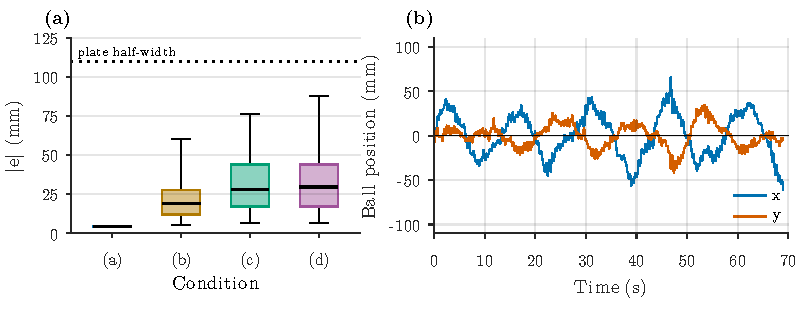
\includegraphics[width=\textwidth]{figures/fig_bp_results.pdf}
  \caption{Left: ball error distribution for conditions (a)--(d) of Table~\ref{tab:bp} (box: quartiles; whiskers: 5th and 95th percentiles). Right: ball position during a ramp run (video \texttt{VID\_20261118\_165747}).}
  \label{fig:bp}
\end{figure}

\paragraph{Discussion}
\begin{itemize}
  \item \textbf{Drone off.} With the drone off, the error is constant at \SI{4.4}{\milli\metre}: the ball settles inside the servo deadband. Vision noise lies well below this level.
  \item \textbf{Rotors at idle.} Turning the rotors on quadruples the median error (to \SI{18.9}{\milli\metre}). The propagation model shows that residual octocopter attitude (within \SI{0.4}{\degree}) accounts for only about \SI{2}{\milli\metre} RMS; the remainder is a slow load acting directly on the ball (rotor downwash, vibration, and backlash), concentrated below \SI{0.3}{\hertz} (Section~\ref{sec:coupling}). With the earlier gains ($k_i=0.2$), the ball fell off in under \SI{5}{\second}; after increasing the integral gain to 0.8, no drops occurred in a \SI{20}{\second} check, and the \SI{469}{\second} trial of condition~(b) completed without drops.
  \item \textbf{Moving base.} Moving the base adds roughly \SI{10}{\milli\metre} to the median and widens the tail (P95 of 76--\SI{88}{\milli\metre}), consistent with the spherical-joint acceleration term in \eqref{eq:balllinx} and its amplification through the octocopter (Fig.~\ref{fig:transm}c). Ramp performance is only slightly worse than flat ground: as \eqref{eq:tilt} predicts, the spherical joint absorbs the \SI{10}{\degree} slope and the octocopter keeps the plate level. With the tray fixed to the base, that same slope would have left the servos only \SI{0.8}{\degree} of usable travel (Section~\ref{sec:porquedron}).
  \item \textbf{Ball detection.} During moving-base runs, the ball was detected 61--100\% of the time. Gaps include drops off the plate edge---often at the ramp transitions, where the accelerometer recorded impacts up to \SI{1.95}{g}---and intervals while the ball was replaced by hand.
\end{itemize}

\begin{figure}[!htbp]
  \centering
  \begin{subfigure}[b]{0.32\textwidth}\centering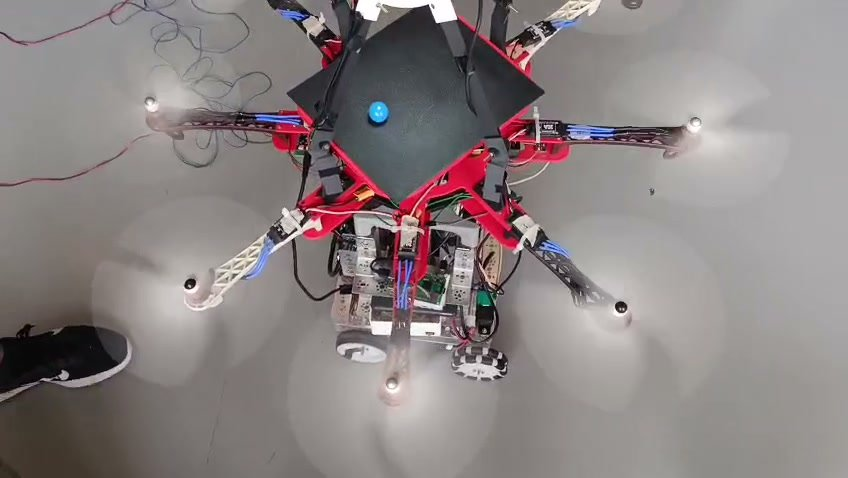
\includegraphics[width=\linewidth]{figures/photo_flat_turn.jpg}\caption{Flat-ground turn.}\end{subfigure}\hfill
  \begin{subfigure}[b]{0.32\textwidth}\centering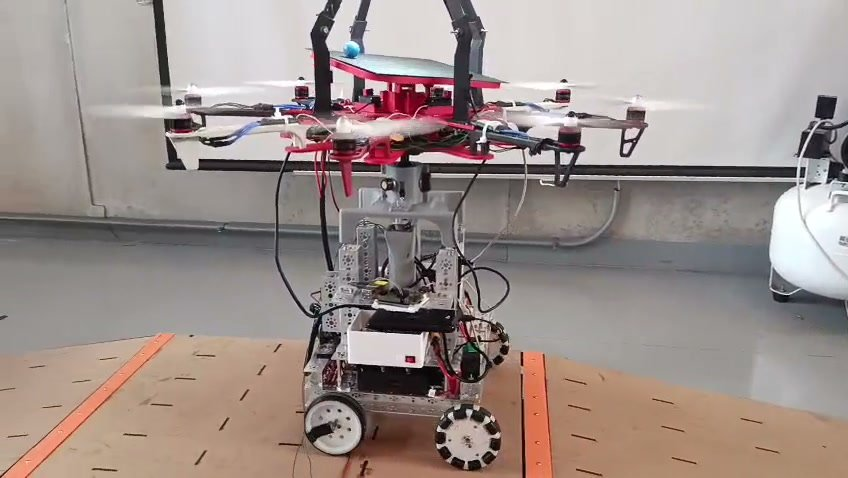
\includegraphics[width=\linewidth]{figures/photo_ramp_climb.jpg}\caption{Climbing the ramp.}\end{subfigure}\hfill
  \begin{subfigure}[b]{0.32\textwidth}\centering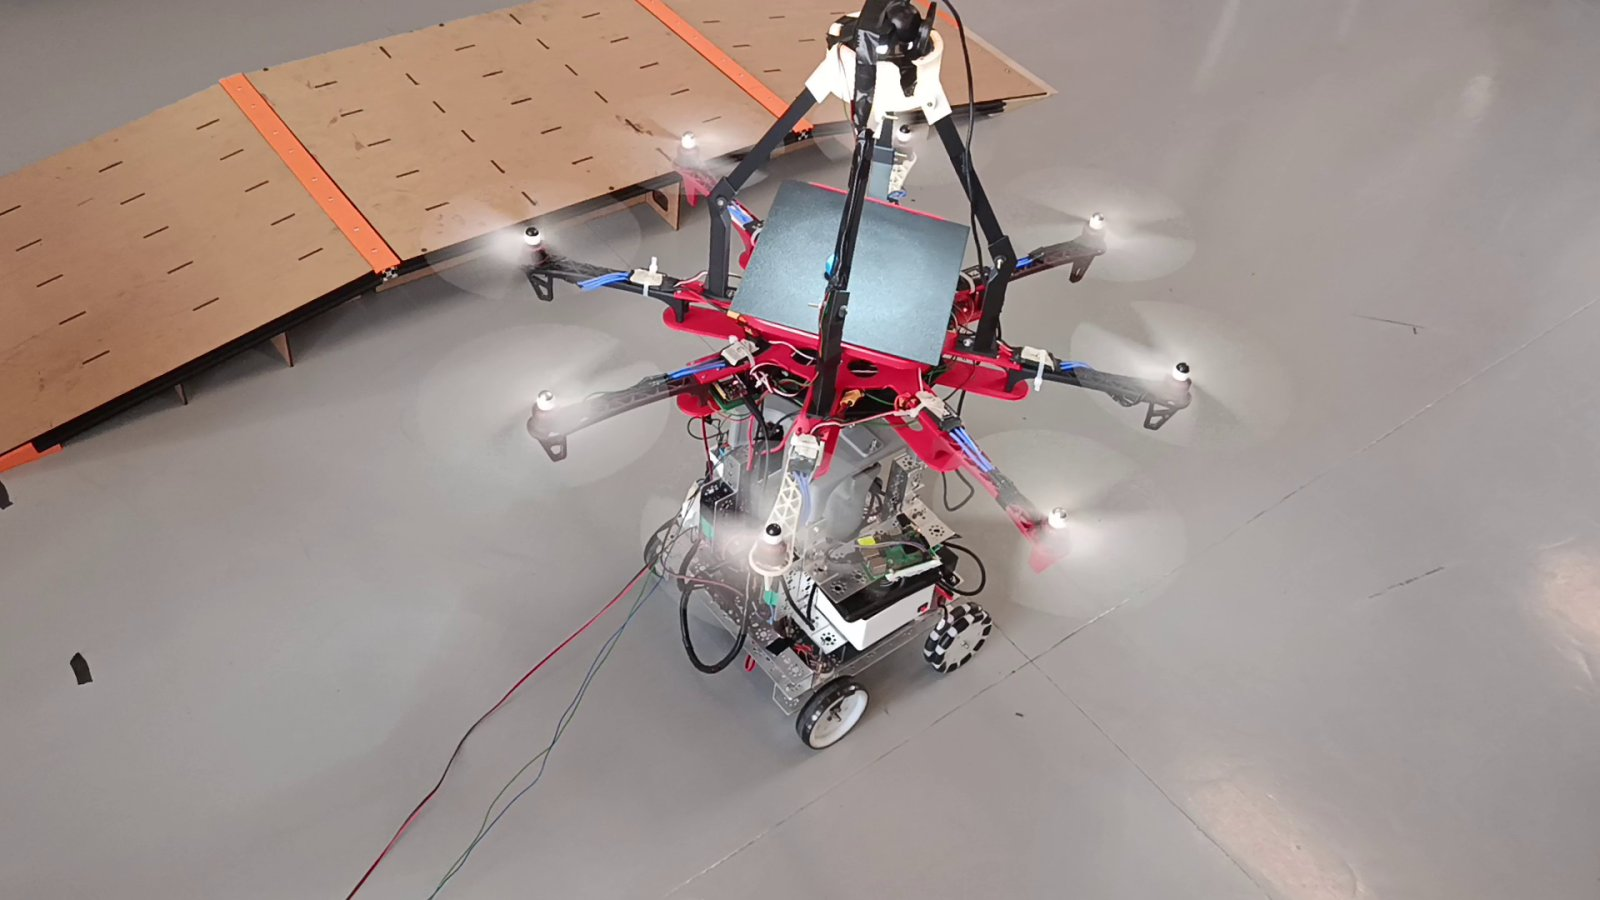
\includegraphics[width=\linewidth,trim=200 0 200 0,clip]{figures/photo_ramp_top.jpg}\caption{At the top of the ramp.}\end{subfigure}
  \caption{Integrated tests on November 18, 2026, with rotors spinning and the ball on the plate (frames from test videos).}
  \label{fig:tests}
\end{figure}

\subsection{Final full-robot trials (Nov.~23)}
\label{sec:ensayos23}
On Nov.~23, ball balancing was repeated on the full robot---the TETRIX mobile base carrying the octocopter on the spherical joint with the ball-and-plate assembly on top---running drone firmware v11 (Sections~\ref{sec:altura} and \ref{sec:metodologia}). We recorded \textbf{13 balancing trials} lasting 23--\SI{122}{\second}, totaling \SI{816}{\second}; in 10 of them, all eight rotors were spinning (\SI{614}{\second}). A trial begins when the PID detects the ball on the plate and ends when the ball leaves the plate or the operator stops it; the first \SI{3}{\second}, during which the ball is placed by hand, are discarded. Table~\ref{tab:ensayos23} and Fig.~\ref{fig:ensayos23} summarize these trials.

\paragraph{Data sources and verification} The Raspberry Pi logged ball position at \SI{187}{\hertz} (\texttt{registro\_20261123\_182316.csv}, 18:23--18:39), but its logs before and after that window could not be downloaded prior to reporting. For those trials, telemetry was recovered from two screen recordings of the web interface (17:29 and 18:36): the page renders the live ball position on the plate map and drone tilt over its 2, 5, and \SI{12}{\degree} rings, and \texttt{extraer\_de\_grabacion.py} measures those markers frame by frame (about \SI{13}{\hertz}) using the page's exact drawing scales. On intervals covered by both the recording and the Pi log, recovered positions differ from logged values by a median of 0.6 and \SI{1.4}{\milli\metre} (P90 of \SI{6.4}{\milli\metre}; 4007 samples), well below the reported errors, so both sources are analyzed together. Screen recovery does not yield servo pulses or drone collective, but it captures plate and motor states.

\begin{table}[!htbp]
\centering
\caption{Ball-balancing trials on the full robot (November 23, 2026). Rot.: rotors spinning. Source: Raspberry Pi log at \SI{187}{\hertz} or telemetry recovered from screen recording. Errors in mm; relative error $e_{\mathrm{RMS}}/R_u$ in \%; effectiveness: \% of time with $e\le\SI{50}{\milli\metre}$. $^\ast$: full-system trial with the base crossing the ramp (Table~\ref{tab:completos23}).}
\label{tab:ensayos23}
\footnotesize
\setlength{\tabcolsep}{3.5pt}
\begin{tabular}{@{}clrclrrrrrc@{}}
\toprule
Trial & Time & $t$ (s) & Rot. & Source & Median & RMS & P95 & Rel.\ err. & Effect. & $\sigma_x$ / $\sigma_y$ \\
 & & & & & & & & & ($\le$\SI{50}{\milli\metre}) & \\
\midrule
01 & 17:30 & 27.0 & yes & video & 29.2 & 33.7 & 56.2 & 34.9 & 88.5 & 30.9 / 11.1 \\
02 & 17:32 & 98.5 & yes & video & 31.8 & 35.3 & 54.9 & 36.6 & 90.5 & 32.3 / 14.3 \\
03 & 17:45 & 122.3 & no & video & 31.5 & 35.0 & 55.7 & 36.3 & 92.1 & 31.2 / 15.7 \\
04 & 18:25 & 22.9 & no & Pi & 44.0 & 51.9 & 94.0 & 53.8 & 63.3 & 49.3 / 11.8 \\
05 & 18:26 & 95.9 & yes & Pi & 39.2 & 51.0 & 99.2 & 52.9 & 67.9 & 49.2 / 13.4 \\
06 & 18:33 & 57.0 & no & Pi & 31.3 & 45.1 & 97.1 & 46.7 & 77.5 & 41.6 / 14.9 \\
07 & 18:36 & 83.5 & yes & Pi & 33.5 & 38.3 & 63.9 & 39.7 & 81.2 & 35.5 / 14.4 \\
08 & 18:40 & 57.4 & yes & video & 42.8 & 46.1 & 72.8 & 47.7 & 65.4 & 40.8 / 20.9 \\
09 & 18:45 & 60.6 & yes & video & 35.1 & 47.3 & 86.5 & 49.0 & 70.2 & 43.4 / 18.8 \\
10$^\ast$ & 18:49 & 39.1 & yes & video & 33.2 & 41.4 & 67.8 & 42.9 & 71.7 & 38.4 / 12.7 \\
11$^\ast$ & 18:51 & 54.7 & yes & video & 42.0 & 48.0 & 82.9 & 49.7 & 67.1 & 38.3 / 28.1 \\
12$^\ast$ & 18:55 & 45.3 & yes & video & 33.4 & 42.6 & 77.4 & 44.1 & 75.7 & 37.2 / 19.6 \\
13$^\ast$ & 19:00 & 51.5 & yes & video & 33.5 & 41.0 & 73.2 & 42.5 & 77.3 & 38.4 / 14.4 \\
\midrule
\multicolumn{5}{@{}l}{Median across 13 trials} & 33.5 & 42.6 & 73.2 & 44.1 & 75.7 & 38.3 / 14.4 \\
\bottomrule
\end{tabular}
\end{table}

\begin{figure}[!htbp]
  \centering
  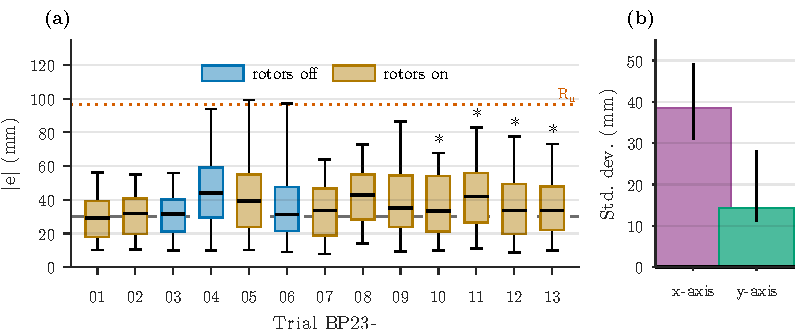
\includegraphics[width=\textwidth]{figures/fig_ensayos_23nov.pdf}
  \caption{Nov.~23 trials on the full robot. (a) Ball error distribution in each trial; the dashed line marks \SI{30}{\milli\metre} and the dotted line marks the usable plate radius. (b) Position standard deviation along each axis (bar: median of the 13 trials; whiskers: minimum and maximum).}
  \label{fig:ensayos23}
\end{figure}

\paragraph{Results}
\begin{itemize}
  \item \textbf{Thirteen continuous balancing segments of 23--\SI{122}{\second} were recorded}, with a median error of 29--\SI{44}{\milli\metre} and 63--92\% of the time within \SI{50}{\milli\metre} of center. The three trials from 17:30--17:47 (BP23-01 to 03) performed best: 29--\SI{32}{\milli\metre} median and 89--92\% of the time within \SI{50}{\milli\metre}, with rotors spinning in two of them. Relative error meets the $\le\SI{45}{\percent}$ criterion of Table~\ref{tab:metricas} in 7 of 13 trials and falls between 46 and \SI{54}{\percent} in the rest; effectiveness in the \SI{30}{\milli\metre} band (25--52\%) does not meet the \SI{60}{\percent} criterion.
  \item \textbf{The rotors do not degrade balancing.} With rotors spinning, drone tilt was 0.71--\SI{1.0}{\degree} RMS, and trials with and without rotors share the same median error (Fig.~\ref{fig:ensayos23}a). The drone kept the plate level across all 10 trials with zero cutoffs.
  \item \textbf{The $x$-axis dominates the error.} Spread along $x$ (31--\SI{49}{\milli\metre}) is 2.7 times that along $y$ (11--\SI{28}{\milli\metre}) in every trial. Along $x$, the ball oscillates side to side with a period of roughly \SI{10}{\second} (Fig.~\ref{fig:bp23despegue}), and the $x$ servo operates with a mean bias of $+65$ to $+\SI{80}{\micro\second}$ above its neutral (\SI{1386}{\micro\second}), reaching its \SI{1612}{\micro\second} stop, whereas the $y$ servo operates centered. This indicates an $x$-axis leveling offset on the plate mounted atop the drone: it consumes one-third of servo travel on that side, and the oscillation is the limit cycle caused by saturation interacting with the integrator. The drone is not the cause, because the same offset appears with the rotors off. Re-leveling the $x$ neutral on the assembled robot (via the Pi's \texttt{/nivelar} routine) directly fixes this.
  \item \textbf{Comparison with Nov.~17--18.} With the base stationary and rotors at idle, the Nov.~17 median was \SI{18.9}{\milli\metre}, compared to 29--\SI{44}{\milli\metre} on Nov.~23. Because the Nov.~23 median $y$-axis spread is \SI{14}{\milli\metre} and the excess error lies in $x$, the difference is attributed to that axis offset, which was absent in earlier sessions.
  \item \textbf{Servo power failure (18:31--18:33).} During this interval, pulse commands varied between 1200 and \SI{1580}{\micro\second}, yet the ball moved less than \SI{0.1}{\milli\metre}: the servo power supply was disconnected. A direct servo check identified the fault, and this interval is excluded from the trials.
\end{itemize}

\paragraph{Full-system trials: base crossing the ramp with drone and ball} In four trials (BP23-10 to 13), the mobile base drove across the \SI{10}{\degree} ramp while the drone---with all eight rotors spinning---leveled the plate and the PID balanced the ball. Motion is confirmed independently in two ways: the LabVIEW screen recording (18:48--19:10, Fig.~\ref{fig:completos23}d) displays the \texttt{ADELANTE} command at 25\% PWM (23\% on the right wheel due to the 0.92 trim) during those intervals, and handheld videos \texttt{VID\_20261123\_184731}, \texttt{\_185130}, \texttt{\_185429}, \texttt{\_190032}, and \texttt{\_190131} (whose filenames encode their start times) show the robot climbing and crossing the ramp transitions (Fig.~\ref{fig:completos23}a--c). Table~\ref{tab:completos23} isolates the moving-base segments.

\begin{table}[!htbp]
\centering
\caption{Nov.~23 full-system trials: base crossing the \SI{10}{\degree} ramp, drone with rotors spinning, and ball balancing. Ball metrics computed only while LabVIEW issued the \texttt{ADELANTE} command.}
\label{tab:completos23}
\small
\begin{tabular}{@{}lrrrrrr@{}}
\toprule
Trial & Moving & Median & P95 & Effect. & Drone RMS & Drone max. \\
 & base (s) & (mm) & (mm) & ($\le$\SI{50}{\milli\metre}) & tilt (\si{\degree}) & tilt (\si{\degree}) \\
\midrule
BP23-10 & 22.9 & 29.6 & 53.7 & 91\,\% & 1.15 & 6.7 \\
BP23-11 & 29.5 & 34.5 & 74.6 & 81\,\% & 0.85 & 4.4 \\
BP23-12 & 18.2 & 30.7 & 52.9 & 89\,\% & 0.99 & 2.3 \\
BP23-13 & 19.0 & 30.6 & 74.7 & 80\,\% & 0.94 & 2.3 \\
\bottomrule
\end{tabular}
\end{table}

\begin{figure}[!htbp]
  \centering
  \begin{subfigure}[b]{0.32\textwidth}\centering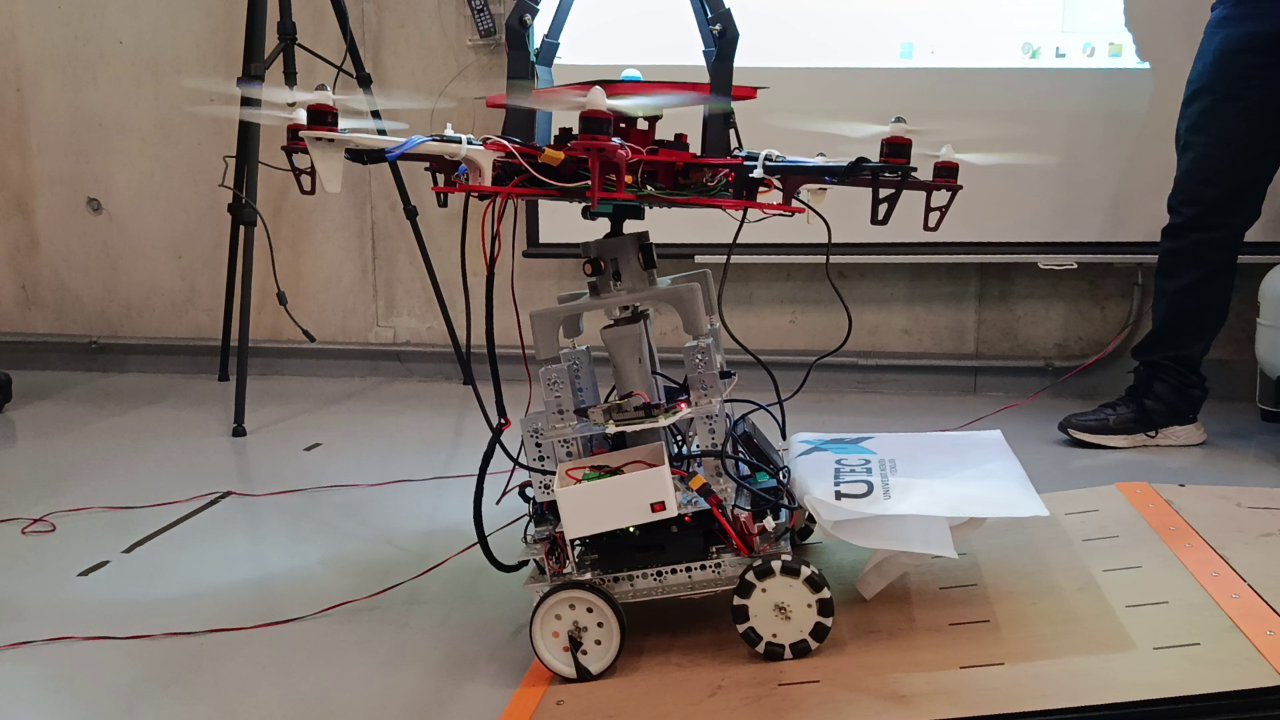
\includegraphics[width=\linewidth]{figures/ensayo23_a.jpg}\caption{BP23-12, 18:55:44.}\end{subfigure}\hfill
  \begin{subfigure}[b]{0.32\textwidth}\centering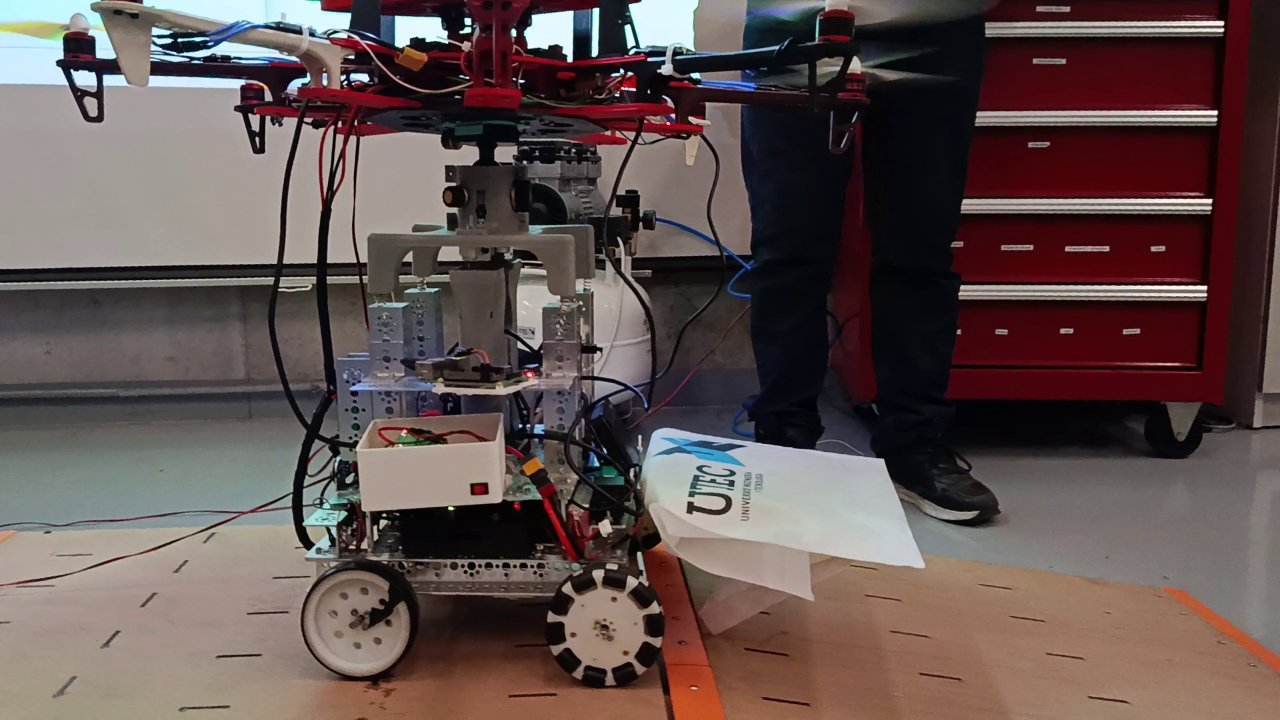
\includegraphics[width=\linewidth]{figures/ensayo23_b.jpg}\caption{BP23-12, 18:55:56.}\end{subfigure}\hfill
  \begin{subfigure}[b]{0.32\textwidth}\centering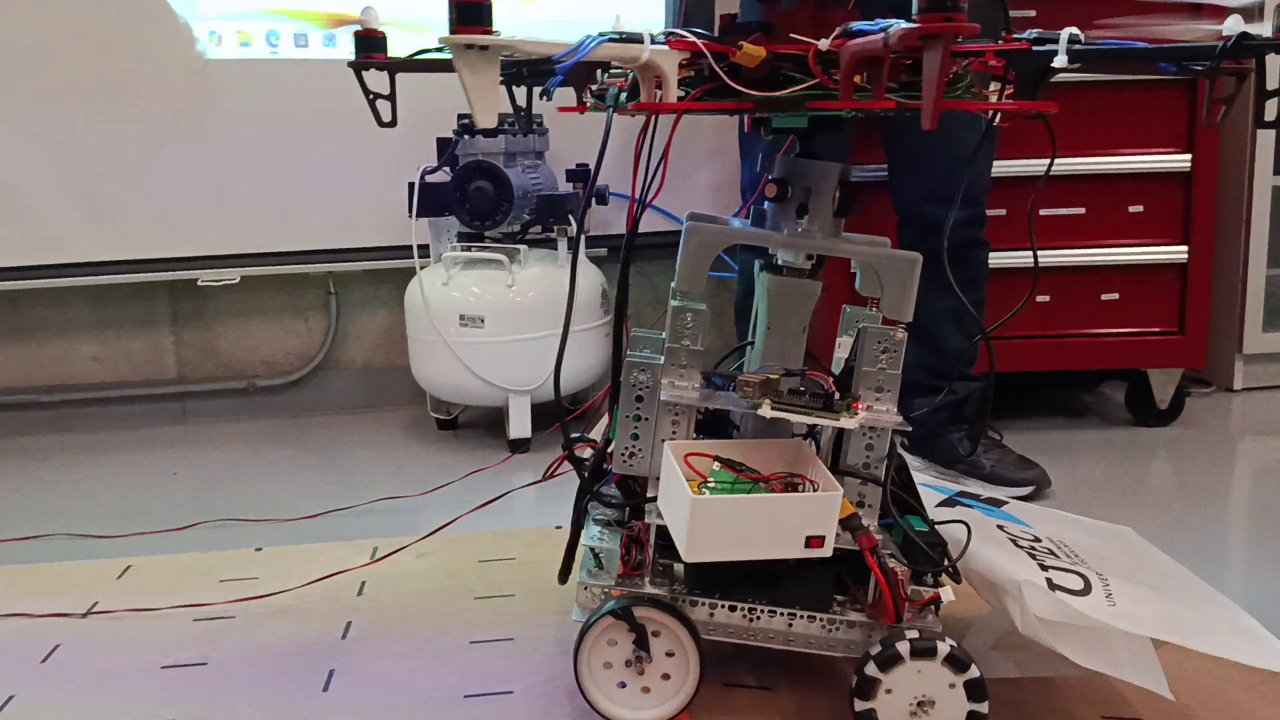
\includegraphics[width=\linewidth]{figures/ensayo23_c.jpg}\caption{BP23-13, 19:01:34.}\end{subfigure}\\[4pt]
  \begin{subfigure}[b]{0.7\textwidth}\centering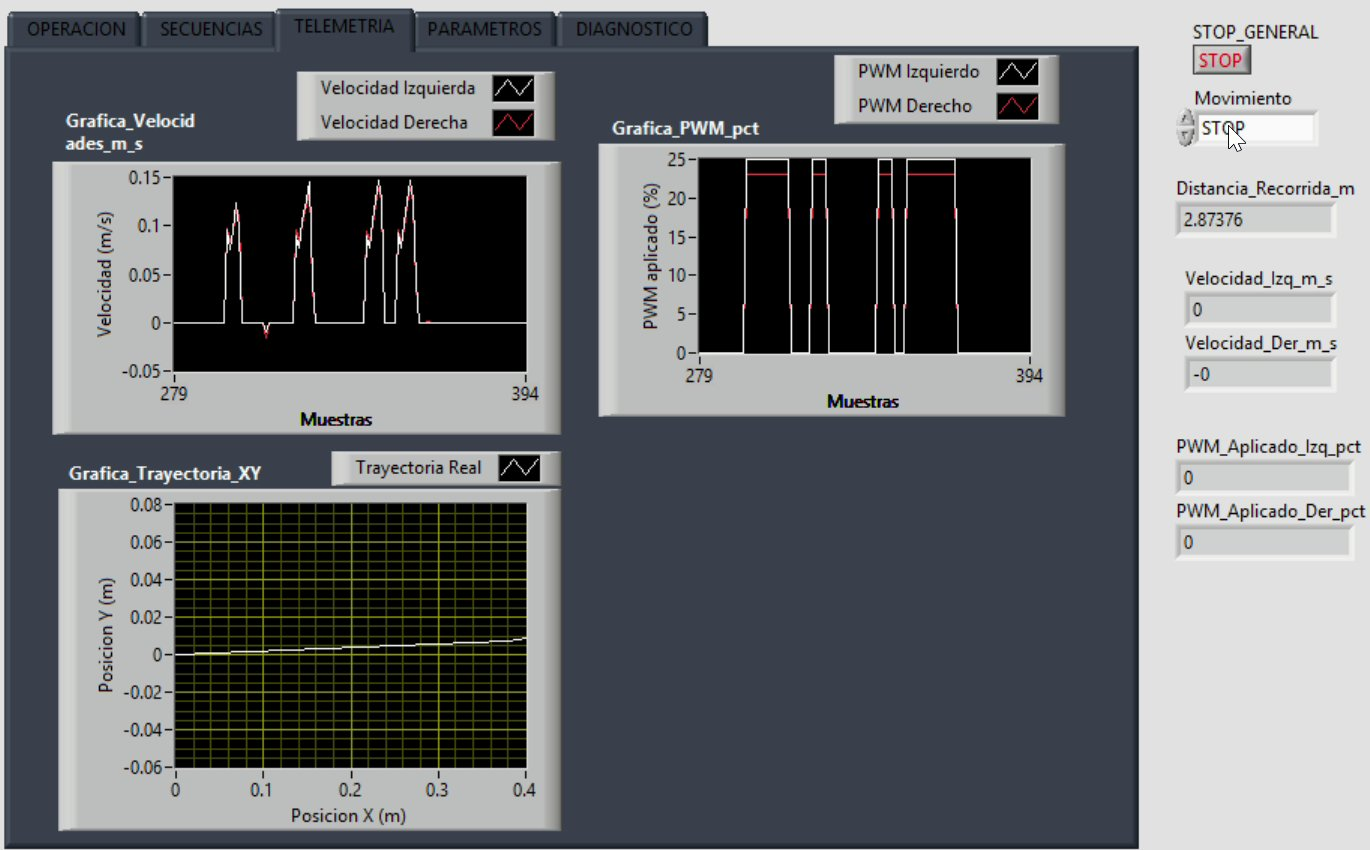
\includegraphics[width=\linewidth]{figures/ensayo23_labview.jpg}\caption{LabVIEW telemetry, 18:49:28.}\end{subfigure}
  \caption{Nov.~23 full-system trials. (a)--(c) The robot crosses the ramp with all eight rotors spinning and the ball on the plate (videos \texttt{VID\_20261123\_185429} and \texttt{\_190131}). (d) myRIO telemetry panel during trial BP23-10: wheel speeds, applied PWM (25/23\,\%), odometry trajectory, and \texttt{ADELANTE} command.}
  \label{fig:completos23}
\end{figure}

During the crossing, the ball stayed within a median of 30--\SI{35}{\milli\metre} from center and 80--91\% of the time within \SI{50}{\milli\metre}---an error equal to or smaller than with the base stationary in the same trials (35--\SI{56}{\milli\metre}) and comparable to the Nov.~18 ramp runs (\SI{29.5}{\milli\metre} median, Table~\ref{tab:bp}). Drone tilt was 0.85--\SI{1.15}{\degree} RMS, with peaks up to \SI{6.7}{\degree} at the transitions, and firmware v11 triggered zero motor cutoffs---unlike the Nov.~18 runs, which ended due to yaw and tilt cutoffs in the bench firmware (Section~\ref{sec:integrated}). The ball stayed on the plate for 18--\SI{30}{\second} of crossing in each trial, on the order of a full traversal of the measured ramp (\SI{2.2}{\metre}; the model predicts \SI{19}{\second} at 25\% PWM, Table~\ref{tab:modelval}). All four trials ended during the crossing as the ball rolled off the plate in the final segment (in BP23-13, while descending the last transition, Fig.~\ref{fig:completos23}c), the same region where drops concentrated on Nov.~18.

\paragraph{Base: speed and straightness} LabVIEW telemetry logged wheel speeds during the Nov.~23 runs. At 25\% PWM, it read 0.078--\SI{0.084}{\metre\per\second} on some segments and 0.124--\SI{0.134}{\metre\per\second} on others. Equation~\eqref{eq:vss} with the measured \SI{10.4}{\kilo\gram} mass predicts \SI{0.078}{\metre\per\second} climbing \SI{10}{\degree} and \SI{0.124}{\metre\per\second} on flat ground, so both groups match the two predictions within 8\%; because telemetry does not flag the current ramp segment, each group is assigned to a segment by proximity. At 40\% PWM, readings ranged from 0.110 to \SI{0.222}{\metre\per\second}, with the peak sitting 8--10\% above the \SI{0.201}{\metre\per\second} flat-ground model prediction. Over a \SI{2.16}{\metre} straight run, odometry ended with \SI{7.8}{\milli\metre} lateral drift (0.4\%) and \SI{-2.7}{\degree} heading error, using the 0.92 right-wheel trim with the wheel PI controller disabled.

\paragraph{Drone takeoff with the ball aboard} In trial BP23-05, hovering was commanded while the ball was balancing (Fig.~\ref{fig:bp23despegue}). The collective ramped from 1300 to \SI{1750}{\micro\second} over \SI{25}{\second} without losing the ball. At 18:28:04, the module lifted off along the vertical guide: the laser reading rose from 385 to \SI{499}{\milli\metre} (a \SI{114}{\milli\metre} climb) with tilt staying within \SI{2.5}{\degree}, and landed cleanly on the land command with zero cutoffs. This was the tenth flight on the guide (the first with firmware v11) and the first carrying the plate and ball. However, the ball---which sat at center ($x=\SI{-1}{\milli\metre}$) half a second earlier---left the plate within \SI{0.5}{\second}: the module jumps upward rather than rising smoothly because guide friction holds it until thrust breaks stiction, and the accelerometer recorded 0.28 to \SI{1.5}{g} at that instant. The plate cannot compensate vertical acceleration, so the fix lies in the takeoff sequence: ramp more slowly near liftoff thrust and engage the cascaded altitude controller (Section~\ref{sec:altura}) as soon as the laser detects upward motion, preventing continued upward acceleration.

\begin{figure}[!htbp]
  \centering
  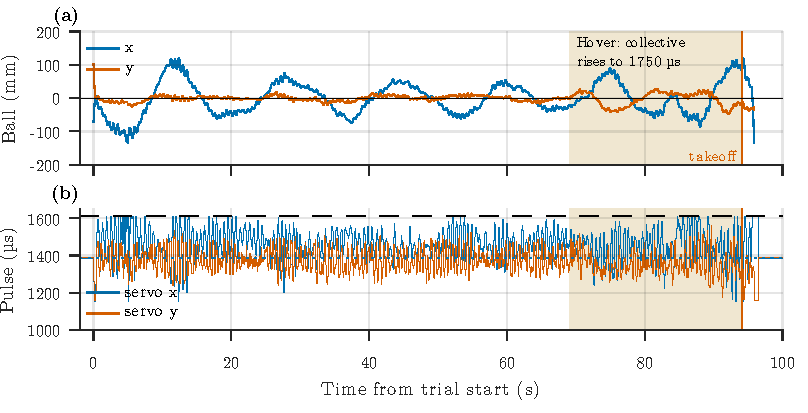
\includegraphics[width=\textwidth]{figures/fig_bp23_despegue.pdf}
  \caption{Trial BP23-05 (Raspberry Pi log at \SI{187}{\hertz}). Top: ball position; bottom: servo pulses, with the $x$-axis neutral (dotted) and upper stop (dashed). The shaded band marks the collective ramp up to \SI{1750}{\micro\second}, and the red line marks drone takeoff, when the ball leaves the plate. Both the slow $x$-axis oscillation and the $x$-servo bias above neutral are visible.}
  \label{fig:bp23despegue}
\end{figure}

\subsection{Mobile base and integrated tests}
\label{sec:integrated}
Fig.~\ref{fig:tests} shows frames from the integrated tests. Carrying the drone with rotors spinning and the ball on the plate, the mobile base completed:
\begin{itemize}
  \item straight runs and turns on flat ground;
  \item climbs and descents of the \SI{10}{\degree} ramp in both directions, repeated over multiple passes (test videos in the repository's \texttt{videos/} folder).
\end{itemize}
In the eight integrated runs of Nov.~18, the drone ran the bench firmware at a \SI{1300}{\micro\second} collective---providing no weight relief ($f\approx0$)---and the runs ended as follows:
\begin{itemize}
  \item four due to the \SI{20}{\degree} yaw cutoff, as the drone rotated with the base;
  \item three due to the \SI{12}{\degree} tilt cutoff, measured at 12.0--\SI{12.2}{\degree} with angular rates up to \SI{49}{\degree\per\second} upon entering the ramp, leaving only \SI{2}{\degree} of margin on a \SI{10}{\degree} slope;
  \item one stopped by the operator.
\end{itemize}
These events confirm the coupling predicted by \eqref{eq:pitchlin}: spherical-joint acceleration at the ramp edges acts on the module through the $-mh_ca_J$ term, and the slow attitude mode amplifies it (Fig.~\ref{fig:transm}b). The UART link between the myRIO and the Pi was implemented on both ends and verified on the Pi using a simulated serial port: valid frames executed, invalid frames were rejected, myRIO priority was respected, and 6-field telemetry was generated. It was then tested with the myRIO connected (Fig.~\ref{fig:uart}): the Pi transmitted ball position over UART, and the myRIO VI received and plotted it in real time on its $x$--$y$ graph, spanning the full plate ($\pm$\SI{150}{\milli\metre}) as the ball moved; the received-character indicator stayed lit throughout the test. In that test, the drone roll and pitch plots remained blank, so drone-to-myRIO telemetry remains to be verified, and the session ended with LabVIEW reporting a lost connection to the myRIO.

\begin{figure}[!htbp]
  \centering
  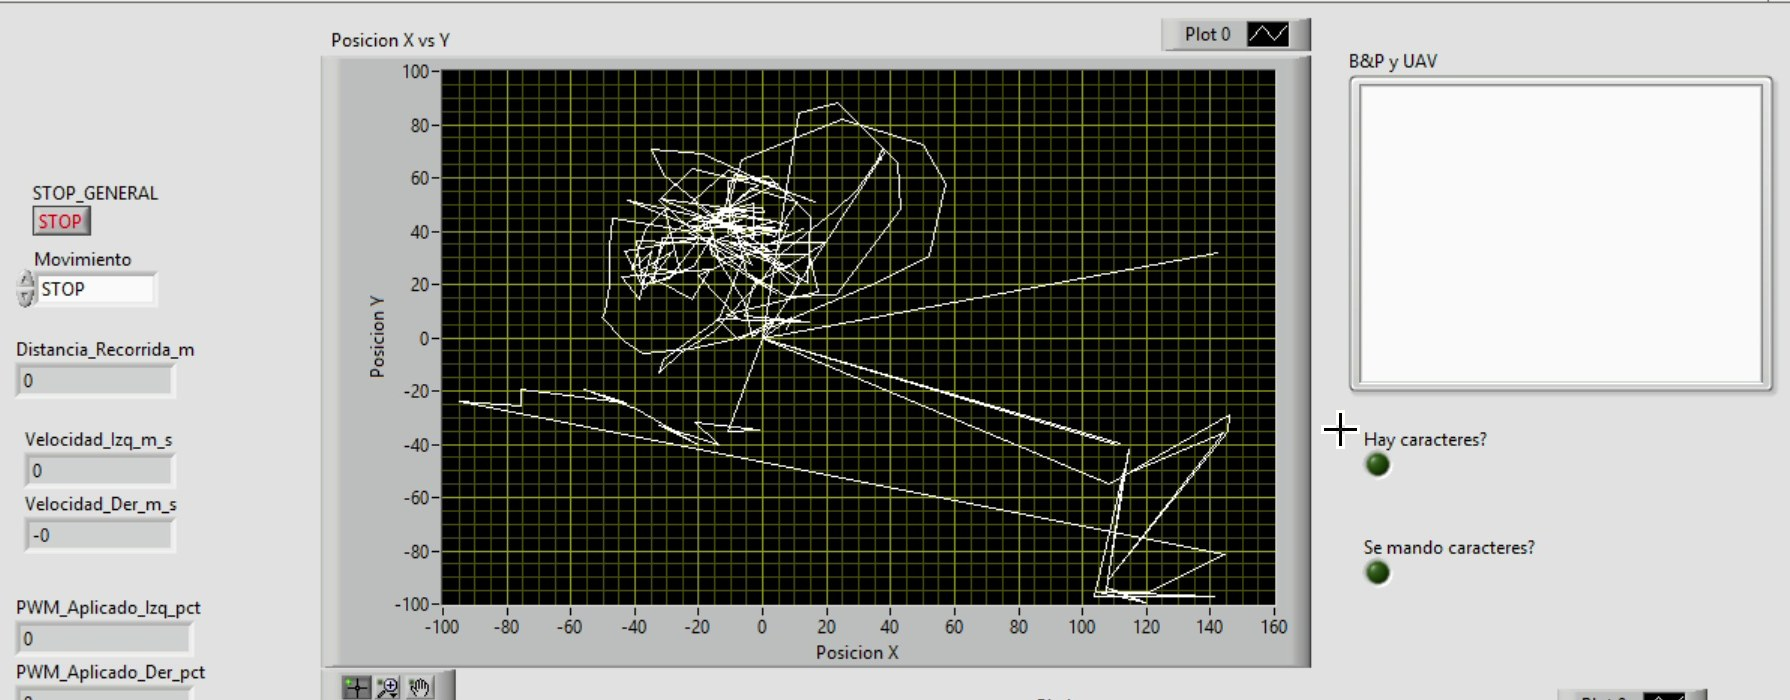
\includegraphics[width=0.9\textwidth]{figures/uart_myrio_bola.jpg}
  \caption{UART link test between the Raspberry Pi and the myRIO: LabVIEW panel showing ball position received from the Pi ($x$--$y$ graph, in mm), the received string (\texttt{B\&P y UAV}), and transmit/receive indicators.}
  \label{fig:uart}
\end{figure}

%% ---- TODO after final base trials: populate and uncomment this table ----
% \begin{table}[!htbp]\centering\small
% \caption{Final base trials (odometry and video). Error = |final position - target|.}
% \begin{tabular}{@{}lrrrr@{}}\toprule
% Trial & Target & Measured (mean $\pm$ SD, $n$) & Error (\%) & Median ball error (mm) \\\midrule
% Translation, flat & 25 cm & & & \\
% Translation, flat & 50 cm & & & \\
% Translation, 10 degrees & 25 cm & & & \\
% Turn about axle midpoint & 360 degrees & & & \\
% Turn about one wheel & 360 degrees & & & \\
% 10-degree climb in ramp mode (f = 0.5) & -- & & & \\
% \bottomrule\end{tabular}\end{table}

\subsection{Model validation}
\label{sec:modelval}
Table~\ref{tab:modelval} compares the predictions of the Section~\ref{sec:model} model against measurements. Parameters identified from a dataset are marked; comparisons in all other rows use data not used to construct the model.

\begin{small}
\setlength{\tabcolsep}{4pt}
\begin{longtable}{@{}>{\raggedright\arraybackslash}p{0.25\textwidth}>{\raggedright\arraybackslash}p{0.22\textwidth}>{\raggedright\arraybackslash}p{0.34\textwidth}>{\raggedright\arraybackslash}p{0.11\textwidth}@{}}
\caption{Model predictions versus measurements.}\label{tab:modelval}\\
\toprule
Quantity & Model & Measurement & Eq./Sec. \\
\midrule\endfirsthead
\toprule Quantity & Model & Measurement & Eq./Sec. \\ \midrule\endhead
Base speed, 15\%, flat & \SI{0.072}{\metre\per\second} & 0.06--\SI{0.08}{\metre\per\second} (LabVIEW telemetry) & \eqref{eq:vss} \\
Base speed, 15\%, \SI{10}{\degree} & \SI{0.027}{\metre\per\second} & ramp climbed more slowly than flat ground (videos) & \eqref{eq:vss} \\
Base speed, 25\%, flat / \SI{10}{\degree} (Nov.~23) & 0.124 / \SI{0.078}{\metre\per\second} & 0.124--0.134 / 0.078--\SI{0.084}{\metre\per\second} (LabVIEW), error $\le\SI{8}{\percent}$ & \eqref{eq:vss} \\
Base speed, 40\%, flat (Nov.~23) & \SI{0.201}{\metre\per\second} & peak 0.217--\SI{0.222}{\metre\per\second} (+8 to +10\%) & \eqref{eq:vss} \\
Hover collective & \SI{1899}{\micro\second} (firmware map); \SI{1770}{\micro\second} (audit) & liftoff at \SIrange{1725}{1775}{\micro\second} & \ref{sec:ident} \\
Takeoff with discharged battery (Flight~9) & \SI{1787}{\micro\second} (1758--1817) & \SI{1796}{\micro\second} & \eqref{eq:ureq} \\
Takeoff at 11.1\,V at rest & 1850--\SI{2000}{\micro\second}: cannot sustain hover & did not hover & \eqref{eq:ureq} \\
Module center of mass & $h_c=\SI{0.10}{\metre}$ (CAD) & $h_c=0.14\pm\SI{0.06}{\metre}$, $\delta_x=9.5\pm\SI{1.8}{\milli\metre}$ (identified) & \eqref{eq:cop} \\
Recoverable tilt, v4--v7 limits & $\theta^\ast=$ 2.8--\SI{3.8}{\degree} & Flights~3--6 drifted to the \SI{12}{\degree} interlock & \eqref{eq:thetastar} \\
Recoverable tilt, v8--v9 limits & $\theta^\ast=$ 16--\SI{19}{\degree} & Flights~7--9 held for 20--\SI{48}{\second} & \eqref{eq:thetastar} \\
Slow attitude mode in hover & 0.20--\SI{0.30}{\hertz}, $\zeta=$ 0.24--0.42 & spectral peaks at 0.15--\SI{0.23}{\hertz} & \ref{sec:attitude} \\
Ball loop, derivative gain & stable at 4.5, unstable at 6 for $K_{b,\mathrm{eff}}=$ 3.5--4.9 & 4.5 stable, 6 unstable (bench) & \ref{sec:ballcontrol} \\
Ball plant gain & 6.0 (CAD); 3.5--4.9 (inferred) & 2.5 / 4.9 ($x$/$y$, regression, $R^2\le0.45$) & \eqref{eq:balltf} \\
Ball error from attitude, rotors on & 1.7--\SI{2.1}{\milli\metre} RMS & 16--\SI{21}{\milli\metre} RMS (dominated by $D_b$) & \eqref{eq:propag} \\
Ball error, stationary vs.\ moving base & increase from base accelerations & median +9 to \SI{11}{\milli\metre} & \eqref{eq:balllinx} \\
Static tip-over angle (locked module) & CAD CoM: $x_G=\SI{81}{\milli\metre}$ & \SI{21.5}{\degree} uphill and \SI{30.5}{\degree} downhill (Nov.~23), giving $x_G=\SI{88}{\milli\metre}$: CAD differs by \SI{8}{\percent} & \eqref{eq:tip} \\
Vertical guide travel & \SI{77}{\milli\metre} (CAD) & about \SI{140}{\milli\metre} (measured) & Table~\ref{tab:params} \\
Spherical joint range vs.\ ramp transitions & required $>\SI{10}{\degree}$ & 35--\SI{53}{\degree} depending on direction & Sec.~\ref{sec:metodologia} \\
Altitude via calibrated laser and Kalman filter & \SI{330}{\milli\metre} (ruler) & 317--\SI{334}{\milli\metre} (error $\le\SI{4}{\percent}$) & \eqref{eq:kfz} \\
Cascaded altitude control & 4--\SI{12}{\milli\metre} peak-to-peak (simulation) & not flight-tested; laser with Kalman filter logged Flight~10 takeoff (\SI{114}{\milli\metre} climb) & \eqref{eq:cascada} \\
Ramp cycle (\SI{0.7}{\metre} at \SI{10}{\degree} + \SI{0.8}{\metre} + \SI{0.7}{\metre}), \SI{15}{\percent} PWM & \SI{41}{\second} at idle; \SI{37}{\second} in ramp mode & pending (stopwatch) & \eqref{eq:vss}, \eqref{eq:descarga} \\
Ramp crossing at \SI{25}{\percent} PWM (Nov.~23) & \SI{19}{\second} & \SI{25.5}{\second} \texttt{ADELANTE} command in BP23-12; ball held 18--\SI{30}{\second} during crossing & \eqref{eq:vss}, \eqref{eq:descarga} \\
\bottomrule
\end{longtable}
\end{small}

The model reproduces every measured quantity, mostly within parameter uncertainty. Its main open discrepancy is the magnitude of the direct ball disturbance, $D_b$, which the model treats as an external input; quantifying rotor airflow over the plate is the natural next experiment. Weight-relief predictions on the ramp have not yet been measured.

\subsection{Requirements compliance and limitations}
\label{sec:requirements}
\label{sec:limits}
Table~\ref{tab:req} compares our results against the validation scenarios in the course guide.

\begin{table}[!htbp]
\centering
\caption{Status of the project guide validation scenarios.}
\label{tab:req}
\footnotesize
\renewcommand{\arraystretch}{1.1}
\begin{tabularx}{\textwidth}{@{}>{\raggedright\arraybackslash}p{0.34\textwidth}>{\raggedright\arraybackslash}X>{\raggedright\arraybackslash}p{0.17\textwidth}@{}}
\toprule
Scenario & Evidence & Status \\
\midrule
Base translation and rotation (flat, \SI{10}{\degree}) & ramp climbed and descended in both directions; Nov.~23 speeds within 8--10\% of model; 0.4\% lateral drift over \SI{2.16}{\metre}; odometry modes for \SI{25}{\centi\metre}, \SI{50}{\centi\metre}, and \SI{360}{\degree} implemented & met for translation; rotation lacks final metric \\
Base on \SI{20}{\degree} slope & not tested; without thrust, measured static tip-over angle is \SI{21.5}{\degree} (\SI{0.26}{\metre\per\second\squared} margin at \SI{20}{\degree}); with ramp mode ($f=0.35$--0.55), margin rises to 0.72--\SI{0.98}{\metre\per\second\squared} (Section~\ref{sec:porquedron}) & not met; feasible with ramp mode, unvalidated \\
Platform and ball estimation & detection at \SI{187}{fps} across the full plate; homography calibration & met \\
Balancing with stationary base & median 4.4 / \SI{18.9}{\milli\metre} (drone off / on, Nov.~17), zero drops; 13 continuous segments of 23--\SI{122}{\second} on Nov.~23 (\SI{816}{\second}, 10 with rotors), median 29--\SI{44}{\milli\metre} (Table~\ref{tab:ensayos23}) & met \\
Balancing during translation (flat, \SI{10}{\degree}) & median 27.9 / \SI{29.5}{\milli\metre} (Nov.~18), P95 below plate half-width; four Nov.~23 full-system ramp crossings with rotors spinning: median 30--\SI{35}{\milli\metre}, 18--\SI{30}{\second} crossing, zero drone cutoffs (Table~\ref{tab:completos23}) & met, with drops on the final ramp segment \\
Balancing during rotation & runs with turns included in condition~(c) & partially met (yaw cutoffs) \\
Intermediate stage (octocopter) & bench RMS $<$\SI{0.4}{\degree}; three hovers on the vertical guide of \SIrange{20}{48}{\second} (Flights~7--9); 0.71--\SI{1.0}{\degree} RMS with rotors and tray aboard (Nov.~23); cutoff-free takeoff and landing with ball aboard (Flight~10, v11) & met on the guide \\
Interface and logging & web interface, LabVIEW panel, CSV logs at camera and drone rates & met \\
\bottomrule
\end{tabularx}
\end{table}

The main limitations are:
\begin{enumerate}[label=(\roman*)]
  \item \textbf{Cutoffs during integrated runs and pending v11 features.} During the Nov.~18 runs, the bench firmware cut off on yaw (\SI{20}{\degree}) and tilt (\SI{12}{\degree}). Firmware v11 resolved the idle yaw cutoff ($\le\SI{1400}{\micro\second}$) via a $\pm\SI{20}{\degree}$ sliding window with a \SI{120}{\degree\per\second} safety ceiling, enabling all four Nov.~23 ramp crossings without cutoffs. Scaling the \SI{12}{\degree} tilt limit with slope and validating active yaw tracking (\texttt{yb}) from the myRIO over full \SI{360}{\degree} turns remain pending.
  \item \textbf{Unmonitored battery voltage.} The firmware does not measure LiPo voltage, yet thrust margin drops with voltage squared: useful sustained flight lasts 3--\SI{7}{\minute} per battery pair, and at 11.1\,V at rest the module no longer lifts off below the sustained limit (Section~\ref{sec:bateria}).
  \item \textbf{Pending protocol tests (future work).} The Nov.~23 campaign did not execute ramp weight relief ($f=0.5$; runs stayed at idle), comparative test~D (locked drone C2 vs.\ free drone C3), tape-measured repetitions of \SI{25}{\centi\metre}, \SI{50}{\centi\metre}, and \SI{360}{\degree} turns (E1), the sinusoidal plate sweep (E2), or the 2 and \SI{5}{\centi\metre} recovery tests (E3).
  \item \textbf{Center of mass and authority margin.} The \SI{9.5}{\milli\metre} eccentricity demands a permanent \SI{0.31}{\newton\metre} trim torque, and the center-of-mass height above the spherical joint ($h_c\approx\SI{0.14}{\metre}$) leaves a small net attitude-loop stiffness (Section~\ref{sec:attitude}).
  \item \textbf{Thrust map.} The thrust map was not identified on a load cell; takeoff data show that $k_F$ is 33--52\% higher than assumed, and its shape at high collective remains unknown.
  \item \textbf{Power system.} The original BMS for the servos and relay coils failed, so a bench power supply was used in part of the tests; GPIO5 and GPIO14 emit startup pulses when the ESP32 boots, requiring the ESCs to be powered only after boot.
  \item \textbf{Vision.} Ball detection relies on color thresholding, so ambient lighting must be controlled.
  \item \textbf{Spherical joint height.} The module center of mass lies above the spherical joint, making the module an inverted pendulum ($h_c=0.14\pm\SI{0.06}{\metre}$, unstable pole at \SI{6.1}{\radian\per\second}) and forcing attitude control near the delay limit $p\theta_e\approx0.5$. Lowering the center of mass below the spherical joint would make it passively stable.
  \item \textbf{Model parameters.} Inertia $\vect J$, base mass distribution, and LiPo internal resistance are estimates derived from CAD, tests, or typical values, and servo lag was inferred rather than measured. A load-cell thrust stand, a bifilar pendulum test for inertia, a servo step-response test, and a loaded voltage-sag measurement would close these gaps.
\end{enumerate}
